\documentclass{ctexart}
\CTEXsetup[format={\Large\bfseries}]{section}            % 让section靠左对齐
\usepackage{graphicx} % Required for inserting images
\usepackage{enumerate} % 下面1,2,3小点


% 设置 subsection 的间距
\usepackage{titlesec}
\titlespacing{\section}{0pt}{0.75\baselineskip}{0.75\baselineskip}
\titlespacing{\subsection}{0pt}{0.5\baselineskip}{0.5\baselineskip}

\usepackage{geometry} % 调整页边距和纸张大小
\geometry{a4paper,scale=0.7} 

\title{\vspace{-2cm}\textbf{程序设计基础课程设计报告} \\ \fontsize{12}{14}{---位图图像文件缩放}}

\author{高宇轩 23009200132}
\date{\today}

\begin{document}
    
    \maketitle
    
    \section{原始题目及要求}
    编写一个程序,可以在命令行输入参数,完成指定文件的缩放,并存储到新文件,命令行参数如下:
    
    zoom file1.bmp 200 file2.bmp
    第一个参数为可执行程序名称;
    
    第二个参数为原始图像文件名;
    
    第三个参数为缩放比例(百分比);
    
    第四个参数为新文件名。
    
    
    \section{题目分析}
    
    \subsection{题目功能}
    将一张位图根据输入的百分比进行缩放,然后将得到的新位图输出到指定文件中。
    
    \subsection{题目知识点}
    文件读写、结构体定义、内存管理、基本图像处理算法、命令行参数
    
    \section{题目总体方案设计}
    
    \subsection{程序功能流程图}
    
    程序功能流程图如图一,主要包括读取位图信息,用压缩算法进行图像处理以及保存位图信息三个模块

    \begin{figure}[h] % 'h' 表示将图片放置在当前位置
        \centering
        
\includegraphics[width=0.8\textwidth]{flow.png}
        \caption{程序功能流程图}  
    \end{figure}

    \subsection{输入输出数据说明}
    输入命令行参数:
    zoom file1.bmp 200 file2.bmp
    
    第一个参数为可执行程序名称;
    
    第二个参数为原始图像文件名;
    
    第三个参数为缩放比例(百分比);
    
    第四个参数为新文件名。
    
    输出新的位图文件。
    
    \subsection{数据结构说明}
    使用<windows.h>头文件中的BITMAPFILEHEADER结构体储存位图文件的文件头;
    
    使用<windows.h>头文件中的BITMAPINFOHEADER结构体储存位图图像的信息块;
    
    使用std::vector<unsigned char>存储位图的像素信息。
    
    
    \section{各功能模块的设计说明}
    \subsection{文件读取}
    要读取bmp文件,我们首先要了解bmp图像的存储格式。BMP位图一般由4部分组成:文件头信息块、图像描述信息块、颜色表(在真彩色模式无颜色表)和图像数据区组成,以BMP为扩展名保存。
    
    因此,我们先读取文件头和文件信息,判断读取的文件是否为24为色深的位图图像,然后计算行的大小并读取像素数据。
    \subsection{压缩算法}
    
    在放大和缩小图片时,我们采用双线性插值作为图像缩放的算法。
    
    双线性插值是一种用于在已知的数据点之间估算其他点数值的方法。当我们要将图像从原始大小缩放到更大或更小的尺寸,而且原始图像的像素不恰好对应到新尺寸的像素上,就需要使用插值方法来估算新尺寸上的像素值,使得图像在缩放或变形能够更加平滑。 
    
    双线性插值的基本思想是,假设我们要在一个矩形区域内估算一个位置的像素值,该位置处于四个已知像素值所确定的矩形的内部。双线性插值首先在水平方向上对两个相邻像素进行线性插值,然后在垂直方向上对得到的两个插值结果进行线性插值,从而得到最终的估算值。
    
    \subsection{文件写入}
    最后,我们依次写入位图文件的文件头,信息头和像素信息,确保位图文件的正确格式。
    
    \section{程序的集成测试}
    在对file1.bmp运行程序后,放大为200\% 得到了file2.bmp,缩小为50\% 得到了file3.bmp。通过文件的大小可以看出,程序实现了放大或缩小位图的功能。
    
    \begin{figure}[h] % 'h' 表示将图片放置在当前位置
        \centering
        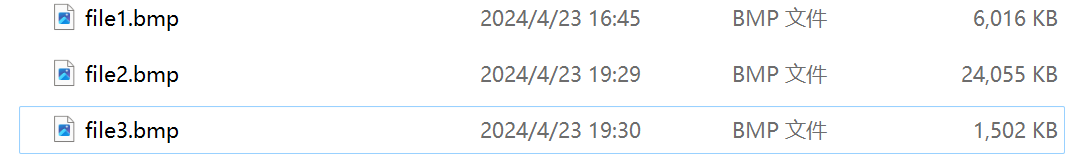
\includegraphics[width=0.8\textwidth]{result.png}
        \caption{程序的集成测试}  
    \end{figure}
    
    \section{总结}
    通过集成测试的结果我们可以看出,我们的程序实现了放大或缩小位图的功能,实现了题目的要求。
    
    另外,我们还可以采用OpenCV的第三方库,更加方便且高效地实现图像的变换。
    
    
\end{document}
